\documentclass{template/openetcs_article}
% Use the option "nocc" if the document is not licensed under Creative Commons
%\documentclass[nocc]{template/openetcs_article} 
\usepackage{lipsum,url}
\usepackage{xspace}
\usepackage{graphicx}
\usepackage{fixme}
\usepackage{lscape} 
\usepackage{pgfgantt}
\usepackage{adjustbox}
\usepackage{datetime}
\usepackage{url}
\usepackage{amsmath}
\usepackage{algorithm}
\usepackage{hyperref}
\usepackage{tikz}
\usetikzlibrary{arrows,automata}

\definecolor{hblue}{RGB}{79,129,189}

%user specified macros


\newcommand{\VV}{Verification \& Validation\xspace}
\newcommand{\vv}{verification \& validation\xspace}

\def\CC{{C\nolinebreak[4]\hspace{-.05em}\raisebox{.4ex}{\tiny\bf ++}}}

\newcommand{\bitwalker}{\mbox{\texttt{Bitwalker}}\xspace}

\newcommand{\poke}{\mbox{\texttt{Bitwalker\_Poke}}\xspace}
\newcommand{\peek}{\mbox{\texttt{Bitwalker\_Peek}}\xspace}
\newcommand{\acsl}{\mbox{\textsf{ACSL}}\xspace}
\newcommand{\isoc}{\mbox{\textsf{C}}\xspace}
\newcommand{\framac}{\mbox{\textsf{Frama-C}}\xspace}
\newcommand{\framacwp}{\mbox{\textsf{Frama-C\slash WP}}\xspace}
\newcommand{\why}{\mbox{\textsf{Why}}\xspace}
\newcommand{\wpframac}{\mbox{\textsf{WP}}\xspace}
\newcommand{\altergo}{\mbox{\textsf{Alt-Ergo}}\xspace}
\newcommand{\qed}{\mbox{\textsf{Qed}}\xspace}
\newcommand{\cvc}{\mbox{\textsf{CVC4}}\xspace}
\newcommand{\z}{\mbox{\textsf{Z3}}\xspace}
\newcommand{\coq}{\mbox{\textsf{Coq}}\xspace}
\newcommand{\cealist}{\mbox{\textsf{CEA LIST}}\xspace}

\newcommand{\inl}[1]{\lstinline[style=inline]{#1}}




\graphicspath{{./template/}{.}{./images/}}
\begin{document}
\frontmatter
\project{openETCS}

%Please do not change anything above this line
%============================
% The document metadata is defined below

\reportnum{OETCS/WP4/D4.2.2}

%define your workpackage or task here
\wp{openETCS@ITEA Work Package 4.2: ``Verification \& Validation of the Formal Model''}

%set a title here
\title{D.4.2.1 1st interim V\&V report on the applicability of the V\&V approach to the formal abstract model}

%set a subtitle here
\subtitle{}

%set the date of the report here
\date{October 2013}

%define a list of authors and their affiliation here
\author{Ana Cavalli \and João Santos}

\affiliation{Télécom SudParis\\
  9 rue Charles Fourier\\
  91011 Evry Cedex, France}
  
% define the coverart
\coverart[width=350pt]{openETCS_EUPL}

%define the type of report
\reporttype{}



%\begin{abstract}
%define an abstract here

%\lipsum[12-13]

%\end{abstract}

%=============================
%Do not change the next three lines
\maketitle
\tableofcontents
\listoffiguresandtables
\newpage
%=============================

% The actual document starts below this line
%=============================


%Start here

\section*{Introduction}

To ensure the correctness and consistency of the model and its implementation, the validation
and verification has to be performed alongside with the modelling process. Thus these tasks will
be performed repeatedly during WP3 and will provide feedback to it.

This document presents the results of the first iteration of verification and validation of the formal model. This was be accomplished
by applying the methods chosen in WP4 Task 1 onto the formal model using the tool
chain developed in WP7. 

This deliverable is a result of the contribution from different partners from the project. The following sections present the contributions of the partners.

\section{Institut Mines-Télécom}

\subsection{Model Based on Extended Timed Finite State Machines}

Over the past century, Europe's railways have been developed within national boundaries, resulting in a variety of different signaling and train control systems, which hampers cross-border traffic. In order to increase interoperability for the railway sector, the European Union has decided to adopt and standardize the European Train Control System (ETCS) new methods and tools to verify the reliability of such system need to be elaborated. Therefore, new techniques for verification and testing of ETCS have to be provided. In this project, we are focusing on using model based testing techniques as formal models are proven to be efficient when testing software and hardware products.
  
In particular, we propose to use finite state machines augmented with continuous variables and guards to represent the most important requirements of the European Train Control System (ETCS) and timeouts. For representing temporal requirements timeouts are used which allow to easily model some critical behavior of the train control system. The above facilities allow describing the basic functioning of the units in this real-time system. At this project step, we are concerned about deriving such model for the ETCS, provide its verification and propose new testing techniques.

The structure of the deliverable is as follows. Section~\ref{sec1} contains the specification of the object being modeled, i.e. the European Train system requirements. The formal specification of such requirements is given in the Section~\ref{sec2}. Methods and tools for model verification are given in Section~\ref{sec3} and~\ref{sec4}, correspondingly. Section~\ref{sec5} refers to a testing problem for an ETCS system.  

\subsection{European Train system requirements}\label{sec1}

The specification of the ETCS system requirements describes the system behavior as well as a number of functional requirements. As the significance and complexity of these requirements grow rapidly, formal techniques for producing reliable control software become of importance. Such formal methods and model-based verification and testing are among the most promising approaches for increasing software confidence.

To formally describe these requirements, one needs a formalism that takes into account continuous variables (variables related to the train position, speed and acceleration) and also different roles of different actors in the specifications: a) the Radio Block Center (RBC), the train (TRAIN), and the environment itself. The devised formal model must represent critical situations such as a) alarm signals from the RBC; b) external inputs to RBC and trains; c) critical distance between two trains; d) the loss of some messages from/to a train or from/to a RBC.  

The following requirements for the train system are considered in the deliverable.

\textit{R1. For each train, there is the safety distance d.}

\textit{R2. If Train$_{id}$ is controlled by the RBC, then the train reports its current position (p), speed (v), and acceleration (a) and the next internal state where the output parameters p, v, a are updated according to the train sensors.}

\textit{R3. “The input parameter SD represents the safety distance between two trains and is a constant in the model.}

\textit{R4. Messages between the train and the RBC may be lost. However, the train continues moving and it should automatically decide if it is in a safe position or not.}

Those four system requirements are taken into account when deriving a formal train system specification which is represented as a timed extended finite state machine.

\subsection{Modeling the European Train System}\label{sec2}

\subsubsection{Formal model for the ETCS}\label{subsec3.1}

\paragraph{Modeling decisions} 

There are many models related to ETCS~\cite{pjesh01,zh05,Ammann2011,ltlzx11,Feuser2012}. Most models describe the system behavior using logic formulas and then verify whether these formulae satisfy some safety requirements, such as the safe distance between trains, alarm messages (fire, accidents, etc.) which can come from outside a train and RBC as well as from inside the train. In order to develop a formal model in the ETCS context it is necessary to consider the actors in Figure~\ref{fig:model} and discuss the behavioral aspects of an RBC and a train under control and which safety aspects should be taken into account. 

\begin{figure}[t!]
\hrule
\sspace

\begin{center}
  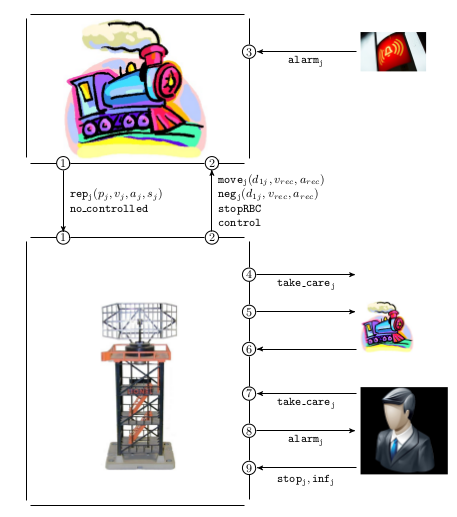
\includegraphics[width=.5\textwidth]{figures/ETCSModel.png}
  \caption{Main Actors in the ETCS.}
  \label{fig:model}
\end{center}
\sspace
\hrule
\end{figure}

1) According to the standards, the ETCS actors communicate in a distributed scenario that is characterized by the absence of a global time, thus, each player has its own clock. Moreover, there are two main safety issues related to time constraints. First, how often the train should report to RBC (position, speed, etc.) and how often the RBC has to send control messages to the train. We do not discuss this issue in the deliverable, since this decision is usually made when verifying the safety of a corresponding logic formula. In our model, this is modeled by discrete time instances when messages may be received/sent. The second aspect is related to the situation when, for some reason, exchange messages are lost. In order to deal with this situation we augment our model with timeout functions. If there is no input before the timeout expires then the player (RBC, a train under control, and/or the environment) has to make their own decision and for the safety issues usually it is the decision to stop the train. Therefore, in our model we synchronize the RBC and train by sending messages with relevant parameters such as the position, the maximum speed, the velocity, or the security point. 

2) Another portion of safety issues is related to situations when a train under control moves in an autonomous way: when the train should negotiate with RBC about the safety distance, when the train should be stopped, i.e., we have to check the functional aspects of the system. Some core points can be defined where an actor has different behaviors, and those points can be considered as states in the model. The conditions when an actor moves from one point (state) to another are usually related to some safety distances between trains, respecting alarm messages, etc. Transitions significantly depend on the values of continuous variables such as train position, speed, acceleration, etc. 

To solve these issues, we consider an ETFSM as a formal model from which tests for verifying the safety aspects of the developed implementations can be automatically generated. According to our model, there are three actors: a train under control, an RBC that also knows the position, speed, acceleration of the previous train, and the environment. The train under control has four special positions where it has different behavior. These positions are depicted in Figure~\ref{fig:states}. 

\begin{figure*}[t]
\hrule
\sspace
\centering
  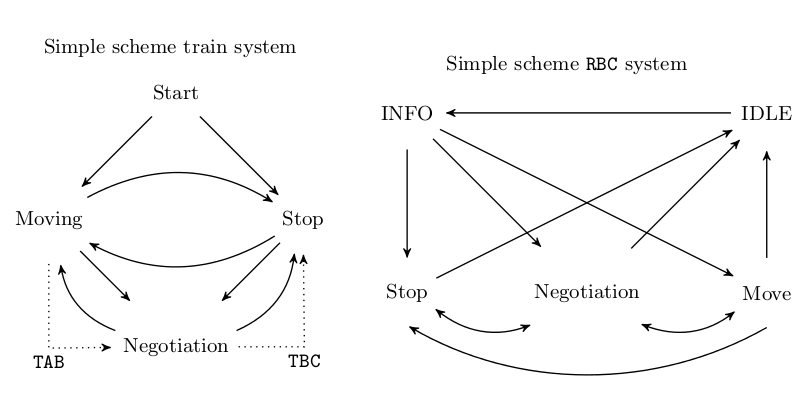
\includegraphics[width=.9\textwidth]{figures/ETCSStates.png}
  \caption{States of the train and \textit{RBC} models.}
  \label{fig:states}
\sspace
\hrule
\end{figure*}

\textbf{Start} The initial state is where the train gets a notification message informing that it is controlled by the given RBC. When getting this message the train reports the corresponding data to RBC and moves to another state (moving/stopping).

\textbf{Moving} At this state, the train can get different messages from RBC but almost any message should contain the safety distance according to the position of the previous train or possibly some obstacles reported to the RBC by the environment. If the train is in a safe position it continues moving in an autonomic way. However, if its position is closer to some dangerous point then the train should come to another state and start the negotiation with RBC.

\textbf{Negot} If the train crosses the dangerous point then the train should be immediately stopped. The safety point can be calculated by the RBC based on the data got from the previous train or on some data got from the environment.

Stop The train is not moving, and it waits for an input of RBC in order to start moving again. In our model, we have such an actor as the environment and as far as we know, the idea of modeling the ETCS environment never has been presented. The environment can send alarm messages to the RBC if something happens outside. We also model the train “red button” (accident, fire etc. inside the train) also by the environment and in this case, the train has to immediately report the situation to the RBC. The RBC states are almost the same as for the train but the RBC can get/send messages to/from the environment that usually is some automatic control (another RBC) or some manager in charge. Moreover, based on the collected information (from other RBC, from trains this RBC is in charge of, etc.) the RBC calculates the safety position for a given train and reports this position to the train. Below we present formula of how this safety position is calculated based on the ETCS requirements.

\paragraph{Modeling requirements}

In this subsection, we briefly describe the main requirements of the ETCS Level 3. In application Level 3 replaces the line-side signals as well as the trackside occupancy checking devices. The location of the train is determined by the trainside optometry and reported to the trackside radio block centre via the GSM-R radio transmission. In this configuration, train spacing is no longer controlled by the interlocking. However, the latter has to exchange information about the route setting with the RBC. In this level, the trains follow the moving block principle~\cite{platzer2009european}, i.e., the current speed and acceleration of a train are dynamically determined by a RBC tracking the train.  Trains are only allowed to move when the RBC grants them permission to do so. According to the set of requirements, in this model, we have the first the \textit{requirement R1} which is the critical point of \textit{Train$_{id}$} of interest (with respect to the previous train). This point is calculated by the RBC that controls the \textit{Train$_{id}$}  to avoid collisions. Figure 1 shows the states which are used in the representations of a train under control and an RBC that controls this train. 

Figure~\ref{fig:model} depicts the actors that are considered in the ETCS, i.e., should be presented in our model, and the exchange messages. The environment actor represents external inputs which may occur in the system, such as an alarm event or a call of an administrator that can interact with the RBC. Thus, the \textit{requirement R2} is also considered in the model.

The RBC analyzes the information obtained from the previous train and returns the critical distance d to the train. According to the rules, the safety distance \textit{requirement R3} is used in the model.

We say that a train at position p and with the critical point d is:

\begin{itemize}
\item In a \textit{safe} position if $(d - p) >= 4 SD$;
\item In a \textit{negotiation} position if $2 SD <=  (d - p) <=  4 SD$;
\item In a \textit{stop} position if $(d - p) < 2 SD$.
\end{itemize}

The developed model takes the above expressions into consideration: If the train is at the \textbf{Moving} state and it is in a \textit{safe} position then it can remain at this state having the speed and acceleration recommended by the RBC that controls the train. However, if the train progresses and the critical distance is not increased with the same speed, then the train will move to a negotiation position and enter the \textbf{Negotiation} state. Finally, if the train is at the \textbf{Negotiation} state and the critical distance does not increase then the train moves to a stop position and enters the \textbf{Stop} state where the train has zero speed. 

Also this Model satisfies the \textit{requirement R4}.

To model this behavior the timeouts $TAB = 4 SD/Vmax$ and $TBC = 2 SD/Vmax$ are introduced in our model (where $Vmax$ is the maximum speed allowed for the train). If the train is at the \textbf{Moving} state and the train does not receive any message from the RBC then after $TAB$ time units it automatically moves to the \textbf{Negotiation} state, while if the train is at the \textbf{Negotiation} state and does not receive any input message from the RBC during TBC then the train moves to the \textbf{Stop} state.

\paragraph{Formal model}

We use the following functions when describing the set of transitions of the train and RBC models:

\begin{itemize}
\item The function $g(RBC)$ returns the critical point $d$ to the \textit{Train$_{id}$};
\item The function $f(Train_{id})$ returns the current position ($p$), speed ($v$) and acceleration ($a$) values and the next internal state of the \textit{Train$_{id}$} according to the values of the train sensors.
\end{itemize}

1) \textbf{The train}: An ETFSM that describes the internal behavior of the Train$_{id}$ has the following states. State \textbf{Start} is the initial state of the train. Any train at this state is not controlled by the RBC of our interest. Once the train is controlled it moves to the \textbf{Moving} state.

The RBC checks the position of the train at appropriate time units which usually are very close to each other. If the train crosses the Negotiation point then the train and the RBC start negotiating and the train moves to \textbf{Negotiation} state. The dot line $TAB$ denotes a timeout. If the train does not receive any input from the RBC during an appropriate time period (this is discussed above), then the train automatically moves to the \textbf{Negotiation} state.  The train is at this state if the train has crossed the Negotiation point but did not reach stop position yet; the RBC calculates a new critical position (point $d$).  If the train reaches Stop position then the train automatically should stop (moves to the \textbf{Stop} state). Otherwise, it continues moving and will go to the \textbf{Moving} state or stay at the \textbf{Negotiation} state depending on the value of $d$ and its current position. At the \textbf{Stop} state the train has the null speed. The train can come to this state if timeouts are triggered or the current position of the train is very close to the critical point, or the train has received an alarm message from inside the train (modeled as a part of the environment) or a \textit{stopRBC} message from the RBC.

2) \textbf{The RBC}: At the initial state \textbf{IDLE}, the RBC collects the information of all the trains which are controlled by this RBC and is waiting for the message \textit{take\_care} to control a train of interest.
 
When the message \textit{take\_care} is confirmed by the train then the RBC moves to the \textbf{Info} state. The \textbf{Info} is the state where the RBC waits for a message from the train that contains its position, speed and acceleration and its current internal state. 

The RBC sends the message \textit{control(k)} to the train in the \textbf{IDLE} state and when $k = j$ the train Train$_j$ is controlled by the RBC. Once getting the message \textit{control(j)} at the \textbf{Start} state the train replies with the message \textit{rep(p; v; a; state)} to the RBC. In fact, once controlled by RBC the train replies with this message to any input from the RBC. The message \textit{move(d; V$_{max}$; a$_{max}$)} sent to the train contains the critical point $d$ (with respect to the previous train or with respect to the next station etc.), the maximum speed $V_{max}$ and the maximum acceleration $a_{max}$ that the train can have. 

Depending on the position of the previous train and possibly other conditions, the critical point $d$ is calculated and according to its value the RBC moves to the \textbf{Stop} state, to the \textbf{Negotiation} state, or to the \textbf{Move} state. The \textbf{Stop} is a state where the RBC finds out that the train is stopped.

It could happen because the position of the train is close to the point $d$ (the train is in a Stop position) or if any external input alarm occurs. The \textbf{Negotiation} is a state that denotes an active exchange of messages between the train and the RBC since the train is not in a \textit{safe} position but did not reach a \textit{stop} position, i.e., the train is in a \textit{negotiation} position. The \textbf{Move} state denotes that the train is moving as autonomous as possible.

The RBC sends the message \textit{stopRBC} in order to stop the train. If the train receives this message at any state then the train moves to the \textbf{Stop} state. 

The message \textit{neg(d; $V_{max}$; $a_{max}$)} is sent to the train when the RBC knows that the train is at the \textbf{Negotiation} state. The environment can send the \textit{alarm} message to the RBC indicating that something is going wrong outside. 

Finally if the RBC gets this message then RBC sends the message \textit{stopRBC} in order to stop this train and enters the \textbf{Stop} state. There is a timeout $TAB$ from state \textbf{Moving} to the \textbf{Negotiation} state, where $TAB = 4 SD$ (four times exceeding the safety distance): 

\textit{If the train is in the \textbf{Moving} state and the train does not receive any input during $TAB$ time units, then the train automatically moves to \textbf{Negotiation} state.}

There also is a timeout $TBC$ from the \textbf{Negotiation} state to the \textbf{Stop} state, where $TBC = 3 SD$ (three times exceeding the safety distance) that means:

\textit{If the train is in the \textbf{Negotiation} state and the train does not receive any input after $TBC$ time units, then it automatically moves to the \textbf{Stop} state.}

\subsubsection{Using specification languages to describe the model}

\paragraph{Using XML and Java for model specification}

In order to assess the possibilities of the model to represent safety properties a prototype in XML-based language has been implemented that was then automatically translated into Java.

A simulator of an EFSM with timeouts has been developed: given a timed parameterized input sequence,  the simulator reproduces the corresponding sequence of outputs. In order to provide a clear representation of the model to the simulator, we depict all components using XML files. In each file, the main component is state and inside each state all its characteristics are presented. Among the possible things, there are transitions that start at this state, internal variables for each state, update functions for these variables and timeouts.  Once the XML file is properly defined, it is parsed in order to create an internal representation of the ETFSM and we use JDOM, a Java library for XML parsing. During this phase, all the components are created internally to be used later for the simulation. After this phase is completed, the model is ready to be executed. The simulator itself is implemented in Java, with a different thread in charge of keeping time (issuing an alarm when a timeout has occurred). Also, each component is represented internally by a different object, for example transitions and timeouts are different object types with very distinct characteristics. 

Nevertheless, to perform model checking we have used different languages to specify the corresponding TEFSM. One of alternative can be the IF language which allows to efficiently specify train safety properties. 

\paragraph{Using IF for model specification}

IF is a language based on temporized machines, allowing the description of existing concepts into specification formalisms.  A real-time system described using IF language is composed of processes running in parallel and interacting asynchronously through shared variables and message exchanges via communication channels. The description of a system in IF consists in the definition of: data types, constants, shared variables, communication signals and processes. In Figure~\ref{fig:if:specification} we represent a short code of the ETCS system in this language.

\begin{figure}[t]
\hrule
\sspace
\centering
  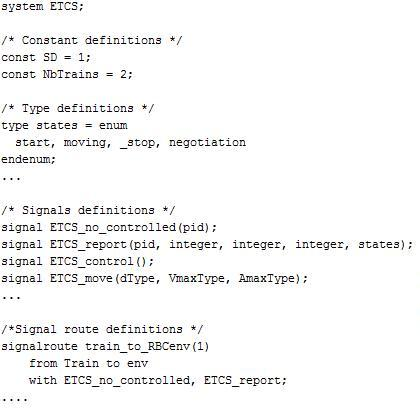
\includegraphics[width=.5\textwidth]{figures/test_generation.jpg}
  \caption{A sample code of the ETCS system specification in IF.}
  \label{fig:if:specification}
\sspace
\hrule
\end{figure}

\paragraph{Using SysML for model specification}

SysML (Systems Modeling Language) is a general-purpose graphical modeling language for systems engineering applications. It supports the specification, analysis, design, verification and validation of a broad range of systems and systems-of-systems. It is defined as an open source specification of a subset extension of the UML, i.e., SysML reuses seven of fourteen diagrams of UML and add two diagrams: requirement and parametric diagrams. It seeks to generalize UML for specifying complex systems that include non-software components such as information, processes, hardware, personnel and facilities.

In this project, we try to use SysML for model specifications. The SysML models are then validated by using SPIN model checker after translating them automatically into Promela.

\subsection{Model verification}\label{sec3}


\subsubsection{Deriving safety properties}\label{subsec3.1}


When performing the verification of the TEFSM model we considered the following safety properties.

\paragraph*{Property 1}

The train is in the \textbf{Moving} state, running at 100km per hour, with an acceleration of 10km per h² on a distance of 100km. Due to some external unexpected reasons, the train must stop as soon as possible. Therefore, an alarm from the environment is sent to the train. Automatically, the train should stop and provide a reporting message with its current parameters (state, position, etc.) to the RBC.

\paragraph*{Property 2}

In this case, the property is the capability of the ETCS system of taking over control if the driver appears to be going too fast.\footnote{This property represents the situation that caused the Spain train accident}  We consider the train in the \textbf{Start} state, receiving the message move with a certain speed and acceleration.

\paragraph*{Property 3}

A train is in the \textbf{Moving} state, running with a speed of 100 km per hour, with an acceleration of 10 km per h², situated somewhere at 10 km from the reference point. The safety distance ($SD$) between two ETCS trains is of 300 km. The train receives the signal move with the maximum speed of 105 km per hour and with an acceleration of 15 km per h² for the next 900 km.

\paragraph*{Property 4}

The property is related to transitions with time-outs. We consider a train in the \textbf{Moving} state, moving with a speed of 100 km per hour, with an acceleration of 10 km per h². The safety distance is of 300 km and the maximum speed allowed is $V_{max} = 105$ km per hour. 

The communication between the train and the RBC is lost, so the train should take an appropriate decision on the next state, after an appropriate period of time.
 
We further discuss different verification techniques that can be used to check the above properties based on the TEFSM.

\subsubsection{Proof technique}

A proof is a demonstration that if some fundamental statements (axioms) are assumed to be true, then some mathematical statement is necessarily true. As mentioned in the requirements document produced by WP2, as much as possible, formal proof would then be used to prove that the OpenETCS model never enter a Feared State, as long as the other subsystem (RBC, communication layer, etc.) fulfill their own safety properties (axiom describing the environment). Such theorem proving helps to increase our confidence on the specified model.  The proof techniques should be integrated in the selected tool chain. In order to use formal proof to verify if the SFM (Semi-formal model) and FFM (fully formal model) comply with the safety and function requirements (cf. R-WP2/D2.6-02-058), the properties to be proven have to be identified and described. There will be a set of axioms that will describe both functional and/or safety properties of the system. The choice of axioms describing functional and/or safety properties will be provided by safety analysis in an independent way from approaches used to specify, design, validate or verify. It must be noted that the model obtained from the Subsystem Requirements Specification should be verified in this manner at a first stage.

\subsubsection{Model checking}

Model checking is an automatic technique for verifying finite-state reactive systems. Using such techniques one could automatically check if the model specifies most of the requirements of the system, such as the important safety properties described in Task 4.4. Similar to proof techniques, in order to use model checking to verify if the SFM (Semi-formal model) and FFM (fully formal model) comply with the safety and function requirements (cf. RWP2 /D2.6-02-058), the properties to be proven have to be identified and described. To implement the use model checking, it is mandatory to specify the model using finite-state reactive systems, and they should also provide an intuitive way to express the properties to be model checked. The language for describing a formal model for which corresponding model checkers exist should be selected and the set of critical requirements to be verified need to be clearly identified. The proposed model checking techniques should be supported in the selected tool chain. As mentioned above, we are using XML-based and IF-based specification to perform the model checking of train safety properties.

\subsubsection{Simulation}

When using model checkers the criteria for the model to be safe all the safety properties should be checked. The latter is impossible, since the number of safety properties is infinite and thus, only some of them can be checked through the above step.

For this reason, as a complementary approach, testing is commonly used. If the corresponding model respects safety requirements, i.e., only expected outputs are produced to applied input sequences, to some extent, there is a confidence that the models is safe. In order to derive ‘good’ tests a formal model should be involved. It is known that only the FSM model where each input is followed by a corresponding output allows automatic deriving finite tests with the guaranteed fault coverage where the races between inputs and outputs can be easily avoided.  Many authors for deriving finite tests with the guaranteed fault coverage turn their model to some kind of an FSM (see, e.g.,~\cite{springintveld2001testing,zymc11,Gromov2009}). 

As for simulation, the artifacts should provide means to execute the model.  The simulator must be automatically generated, so that, when run against test scenarios (inputs/outputs for the model), we may conclude whether the model follows the specification or not. In particular, it is important to define test scenarios for the safety critical properties. Since, the developmentwithin openETCS has to the goal to reach the CENELEC EN 50128 SIL 4 standard, it is highly recommended (cf. SIL 4) that the simulation needs to cover all states, transitions, data-flow, and paths in the model. It would also be desirable to include graphical representation of the simulation/model and also provide a report of the visited components as specified by CENELEC EN 50128 SIL 4. CENELEC EN 50128 SIL4 also advocates to perform tracing. Being able to trace the requirements that are met during a simulation is also advisable to allow simple requirement coverage.

\subsubsection{Other Methods}

Reviews, Inspections, static analysis and walkthroughs, mostly manual techniques, are also to be considered for the verification of models. 

\subsection{Existing software tools for model verification}\label{sec4}

\subsubsection{SPIN model checker}

SPIN (Simple Promela INterpreter)~\cite{Holzmann97} is an open-source software too1, written in C, for simulating and verifying concurrent systems. The communications, via message channels, between concurrent processes of system can be synchronous, i.e., rendezvous, or asynchronous, .i.e., buffered. Models of systems to be analyzed are described by Promela (PROcess MEta LAnguage). In simulation mode, the model is executed step-by-step to familiarize with the behaviors of system. In verification mode, the model is exhaustively explored in order to show that it satisfies some critical properties, e.g., deadlock-free, violated assertions, or general correctness requirements given in Linear Temporal Logic formulas. In this mode, SPIN generates a C program that constructs an implementation of the model-checking algorithm for the given model. The program is then compiled and run to get the result.

As SPIN is proven to be efficient model checker we further plan to try a model checking approach using Promela specification. For this purpose, we will derive a Promela specification from of the TEFSM and perform the model checking of safety properties. Such safety properties will be specified as assertions, and corresponding violations will provide the counter-examples if the model will be invalid.

\subsubsection{Using JPF model checker}

Java Pathfinder~\cite{JPF} is a system to verify executable Java bytecode programs. The core of JPF is a Java Virtual Machine that is also implemented in Java. JPF executes normal Java bytecode programs and can store, match and restore program states. Its primary application has been Model checking of concurrent programs, to find defects such as data races and deadlocks. 

As in this project, the XML-specification of the train system is automatically converted into Java code we also consider to use this model checker in the future. In this case, safety properties will be specified as Java assertions and will be added to the corresponding Java implementation. 

\subsection{Testing European Train System}\label{sec5}

\subsubsection{Adaptive scenario} 

In this section, we present the notion of testing and discuss a testing scenario for our model. We assume that the RBC and the train are tested separately, i.e., when testing the train software the RBC is replaced by a tester that sends inputs to the train and checks whether the produced outputs are expected. Moreover, we consider adaptive testing, i.e., a test case is represented as an acyclic ETFSM~\cite{Petrenko2011,offutt1989coupling} where only one timed input is defined at each intermediate state. We start at the initial state and apply an input defined at the state to an IUT. Based on the produced output the FSM R that represents a test case will move to another prescribed state where another input can be specified and exactly this input will be applied at the next step.  If the observed trace is a trace of the specification TEFSM then we say that the IUT passed a test case. Otherwise, the IUT fails the test case, i.e., the IUT does not conform to the given specification. We illustrate our approach using the following testing scenario (Figure~\ref{testing:scenario}):

\begin{figure}[t!]
\hrule
\sspace

\begin{minipage}{0.3\hsize}
\centering
\textbf{Step 1}\\

	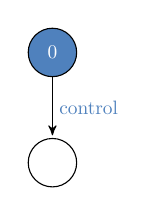
\begin{tikzpicture}[>=stealth',shorten >=1pt,auto,node distance=2cm,scale=0.7, every node/.style={scale=0.7}]
	  \node[state, fill=hblue, text=white] (A)      {$0$};
	  \node[state]         (B) [below of=A]  {};
	 
	 
	  \path[->] 
		(A) edge  node [hblue] {control} (B)
	;
	\end{tikzpicture}

\end{minipage}
\begin{minipage}{0.7\hsize}

\textbf{Step 2}\\

	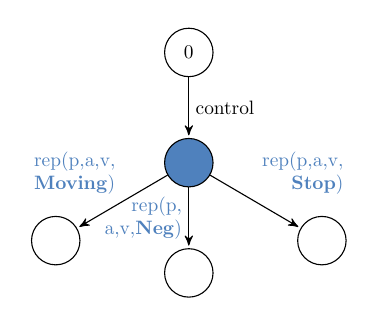
\begin{tikzpicture}[>=stealth',shorten >=1pt,auto,node distance=2cm,scale=0.7, every node/.style={scale=0.7}]
	  \node[state] (A)      {$0$};
	  \node[state, fill=hblue]         (B) [below of=A]  {};
	  \node[state]         (C) [below left of=B,xshift=-1cm]  {};
	  \node[state]         (D) [below of=B]  {};
	  \node[state]         (E) [below right of=B,xshift=1cm]  {};
	 
	 
	  \path[->] 
		(A) edge  node {control} (B)
		(B) edge  node [hblue,align=left, above left] {rep(p,a,v,\\\textbf{Moving})} (C)
		(B) edge  node [hblue, align=right, left ] {rep(p,\\ a,v,\textbf{Neg})} (D)
		(B) edge  node [hblue, align=right] {rep(p,a,v,\\\textbf{Stop})} (E)
	;
	\end{tikzpicture}

\end{minipage}

%\begin{minipage}{1\hsize}


\centering
	\textbf{Step 3}\\

	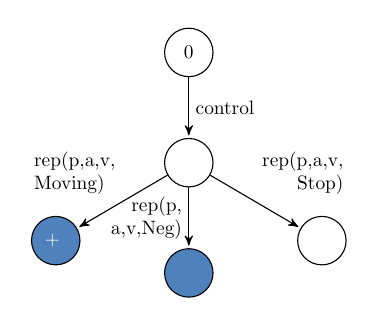
\begin{tikzpicture}[>=stealth',shorten >=1pt,auto,node distance=2cm,scale=0.7, every node/.style={scale=0.7}]
	  \node[state] (A)      {$0$};
	  \node[state]         (B) [below of=A]  {};
	  \node[state, fill=hblue, text=white]         (C) [below left of=B,xshift=-1cm,align=center]  {\TAB + \TBC};
	  \node[state, fill=hblue, text=white]         (D) [below of=B]  {\TBC};
	  \node[state]         (E) [below right of=B,xshift=1cm]  {};
	 
	 
	  \path[->] 
		(A) edge  node {control} (B)
		(B) edge  node [align=left, above left] {rep(p,a,v,\\Moving)} (C)
		(B) edge  node [align=right, left ] {rep(p,\\ a,v,Neg)} (D)
		(B) edge  node [align=right] {rep(p,a,v,\\Stop)} (E)
	;
	\end{tikzpicture}

\textbf{Step 4}\\

	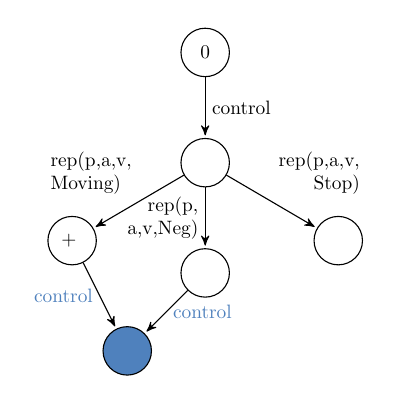
\begin{tikzpicture}[>=stealth',shorten >=1pt,auto,node distance=2cm,scale=0.7, every node/.style={scale=0.7}]
	  \node[state] (A)      {$0$};
	  \node[state]         (B) [below of=A]  {};
	  \node[state]         (C) [below left of=B,xshift=-1cm,align=center]  {\TAB + \TBC};
	  \node[state]         (D) [below of=B]  {\TBC};
	  \node[state]         (E) [below right of=B,xshift=1cm]  {};
	  \node[state, fill=hblue]		   (F) [below left of=D] {};
	 
	 
	  \path[->] 
		(A) edge  node {control} (B)
		(B) edge  node [align=left, above left] {rep(p,a,v,\\Moving)} (C)
		(B) edge  node [align=right, left ] {rep(p,\\ a,v,Neg)} (D)
		(B) edge  node [align=right] {rep(p,a,v,\\Stop)} (E)
		(C) edge  node [hblue, left] {control} (F)
		(D) edge  node [hblue, right] {control} (F)
	;
	\end{tikzpicture}


%\end{minipage} 
%\begin{minipage}{0.3\hsize}

\centering
		\textbf{Step 5}

	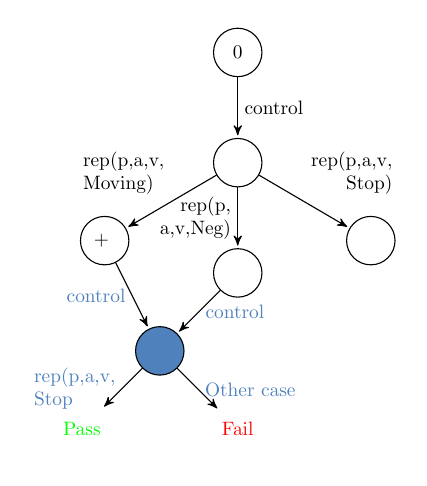
\begin{tikzpicture}[>=stealth',shorten >=1pt,auto,node distance=2cm,scale=0.7, every node/.style={scale=0.7}]
	  \node[state] (A)      {$0$};
	  \node[state]         (B) [below of=A]  {};
	  \node[state]         (C) [below left of=B,xshift=-1cm,align=center]  {\TAB + \TBC};
	  \node[state]         (D) [below of=B]  {\TBC};
	  \node[state]         (E) [below right of=B,xshift=1cm]  {};
	  \node[state, fill=hblue]		   (F) [below left of=D] {};
	 \node[state]		   (G) [below left of=F, white, text=green] {Pass};
	 \node[state]		   (H) [below right of=F, white, text=red] {Fail};
	 
	  \path[->] 
		(A) edge  node {control} (B)
		(B) edge  node [align=left, above left] {rep(p,a,v,\\Moving)} (C)
		(B) edge  node [align=right, left ] {rep(p,\\ a,v,Neg)} (D)
		(B) edge  node [align=right] {rep(p,a,v,\\Stop)} (E)
		(C) edge  node [hblue, left] {control} (F)
		(D) edge  node [hblue, right] {control} (F)
		(F) edge  node [hblue, left, align=left] {rep(p,a,v,\\Stop} (G)
		(F) edge  node [hblue, right] {Other case} (H)
	;
	\end{tikzpicture}

%\end{minipage}

\caption{Testing scenario.\label{testing:scenario}}
\sspace
\hrule
\end{figure}


\textit{If there is no signal from RBC (lost messages) for an appropriate period of time then a train must stop itself.}

In Figure~\ref{testing:scenario} are represented the following five steps:

\begin{enumerate}
\item The tester (simulating the RBC functioning) starts with sending the message control to the train. The 0 value in the initial state means that the RBC does not wait anything to send this message.
\item Depending on the internal state of the train, the tester moves to different states. In order to simplify the example let us consider that the train always answers this message.
\item At these states the tester waits for the appropriate number of time units $TAB + TBC$ or $TBC$ when there are no messages sent to the train.
\item Then the tester checks the state of the train by sending the control message again.
 If the train is in the \textbf{Stop} state then the tester returns \textit{Pass}, otherwise it returns \textit{Fail}. Finally, having the train at the \textbf{Stop} state the tester forces it to move with the maximal permissible speed and acceleration and returns the critical distance $d$.
\end{enumerate}
 
In the same way, other testing scenarios for checking safety properties may be considered. For example, we can derive a test case that checks whether a train stops when being close to the critical point $d$, a test case that checks whether a train changes the Moving state when crossing the critical point $d$, a test case that checks whether a train speed (acceleration) does not exceed the permissible maximum, etc. Finally, it is worth mentioning that when we are testing whether a train stops when reaching a critical point or whether the train respects RBC requirements about its speed and acceleration we must use continuous variables.

\subsubsection{Test generation based on IF representation}

In this Section we present how to automatically extract a set of tests from the specification. To do this, the behavior of the train process is described in the IF language. We have identified a set of basic requirements and we can describe them as properties in IF.  Based on these properties, the validation and verification of the formal specification are carried out using the IF toolset TestGen-IF which automatically generate a set of adaptive tests.

We present a short overview of the result of applying this tool in a requirement related to Property 1 (Section~\ref{subsec3.1}). The set of test objectives associated to this scenario, noted as OBJ(1) is formally described in Figure~\ref{set:of:tests}.

\begin{figure}[t]
\hrule
\sspace

\begin{lstlisting}
#Test-case for the train in the Moving state
?ETCS_control{}!ETCS_report{{Train}0,10,100,10,start}
?ETCS_alarm_to_train{}!ETCS_report{{Train}0,10,
	100,10,moving}
?ETCS_control{} !ETCS_report{{Train}0,10,0,0,_stop}
#Test-case for the train in the Negotiation state
?ETCS_control{}!ETCS_report{{Train}0,10,100,10,start}
?ETCS_move{900,105,15}!ETCS_report{{Train}0,10,100,
	10,moving}
?ETCS_alarm_to_train{}!ETCS_report{{Train}0,10,100,
	10,negotiation}
?ETCS_control{}!ETCS_report{{Train}0,10,0,0,_stop}
\end{lstlisting}
\caption{Set of test using TestGen IF tool.\label{set:of:tests}}
\sspace
\hrule

\end{figure}


Let us note that, according to the system specification, the property OBJ(1) is correct in any of the states of the train model. Therefore, at any state, the train should stop when receiving an external alarm input.

Different test scenarios are performed with respect to safety properties discussed in Section~\ref{subsec3.1}. As a future work we plan to verify the fault coverage of these tests by executing Java simulator against corresponding traces.


\subsection*{Results}

In this deliverable, we have provided a formal model for the requirements of the European Train Control System using finite state machines augmented with continuous variables (train position, speed, acceleration) and time constraints. The model is a very close representation of the system specification provided by the standard.

We have discussed different model checking techniques to verify safety properties for corresponding TEFSM representing the ETCS. To efficiently perform such model checking we use different specification languages, namely, XML and IF languages.
%
We have proposed a technique of the ETCS adaptive testing w.r.t. test scenarios written as train safety properties. 

As a future work, we plan to use different model checkers and perform experiments with the model being derived. We plan to use SPIN and for this purpose we will specify the TEFSM in the SysML language that will be further translated into Promela. Meanwhile, we plan to use the JPF model checker to efficiently utilize the Java train simulator that has been developed during the first part of the project.

\nocite{*}
%===================================================
%Do NOT change anything below this line

%\bibliographystyle{IEEEtran}
\bibliographystyle{unsrt}

\bibliography{biblio}
%

\end{document}
